\documentclass[twoside]{book}

% Packages required by doxygen
\usepackage{fixltx2e}
\usepackage{calc}
\usepackage{doxygen}
\usepackage[export]{adjustbox} % also loads graphicx
\usepackage{graphicx}
\usepackage[utf8]{inputenc}
\usepackage{makeidx}
\usepackage{multicol}
\usepackage{multirow}
\PassOptionsToPackage{warn}{textcomp}
\usepackage{textcomp}
\usepackage[nointegrals]{wasysym}
\usepackage[table]{xcolor}

% Font selection
\usepackage[T1]{fontenc}
\usepackage[scaled=.90]{helvet}
\usepackage{courier}
\usepackage{amssymb}
\usepackage{sectsty}
\renewcommand{\familydefault}{\sfdefault}
\allsectionsfont{%
  \fontseries{bc}\selectfont%
  \color{darkgray}%
}
\renewcommand{\DoxyLabelFont}{%
  \fontseries{bc}\selectfont%
  \color{darkgray}%
}
\newcommand{\+}{\discretionary{\mbox{\scriptsize$\hookleftarrow$}}{}{}}

% Page & text layout
\usepackage{geometry}
\geometry{%
  a4paper,%
  top=2.5cm,%
  bottom=2.5cm,%
  left=2.5cm,%
  right=2.5cm%
}
\tolerance=750
\hfuzz=15pt
\hbadness=750
\setlength{\emergencystretch}{15pt}
\setlength{\parindent}{0cm}
\setlength{\parskip}{3ex plus 2ex minus 2ex}
\makeatletter
\renewcommand{\paragraph}{%
  \@startsection{paragraph}{4}{0ex}{-1.0ex}{1.0ex}{%
    \normalfont\normalsize\bfseries\SS@parafont%
  }%
}
\renewcommand{\subparagraph}{%
  \@startsection{subparagraph}{5}{0ex}{-1.0ex}{1.0ex}{%
    \normalfont\normalsize\bfseries\SS@subparafont%
  }%
}
\makeatother

% Headers & footers
\usepackage{fancyhdr}
\pagestyle{fancyplain}
\fancyhead[LE]{\fancyplain{}{\bfseries\thepage}}
\fancyhead[CE]{\fancyplain{}{}}
\fancyhead[RE]{\fancyplain{}{\bfseries\leftmark}}
\fancyhead[LO]{\fancyplain{}{\bfseries\rightmark}}
\fancyhead[CO]{\fancyplain{}{}}
\fancyhead[RO]{\fancyplain{}{\bfseries\thepage}}
\fancyfoot[LE]{\fancyplain{}{}}
\fancyfoot[CE]{\fancyplain{}{}}
\fancyfoot[RE]{\fancyplain{}{\bfseries\scriptsize Generated by Doxygen }}
\fancyfoot[LO]{\fancyplain{}{\bfseries\scriptsize Generated by Doxygen }}
\fancyfoot[CO]{\fancyplain{}{}}
\fancyfoot[RO]{\fancyplain{}{}}
\renewcommand{\footrulewidth}{0.4pt}
\renewcommand{\chaptermark}[1]{%
  \markboth{#1}{}%
}
\renewcommand{\sectionmark}[1]{%
  \markright{\thesection\ #1}%
}

% Indices & bibliography
\usepackage{natbib}
\usepackage[titles]{tocloft}
\setcounter{tocdepth}{3}
\setcounter{secnumdepth}{5}
\makeindex

% Hyperlinks (required, but should be loaded last)
\usepackage{ifpdf}
\ifpdf
  \usepackage[pdftex,pagebackref=true]{hyperref}
\else
  \usepackage[ps2pdf,pagebackref=true]{hyperref}
\fi
\hypersetup{%
  colorlinks=true,%
  linkcolor=blue,%
  citecolor=blue,%
  unicode%
}

% Custom commands
\newcommand{\clearemptydoublepage}{%
  \newpage{\pagestyle{empty}\cleardoublepage}%
}

\usepackage{caption}
\captionsetup{labelsep=space,justification=centering,font={bf},singlelinecheck=off,skip=4pt,position=top}

%===== C O N T E N T S =====

\begin{document}

% Titlepage & ToC
\hypersetup{pageanchor=false,
             bookmarksnumbered=true,
             pdfencoding=unicode
            }
\pagenumbering{alph}
\begin{titlepage}
\vspace*{7cm}
\begin{center}%
{\Large Node Framework }\\
\vspace*{1cm}
{\large Generated by Doxygen 1.8.14}\\
\end{center}
\end{titlepage}
\clearemptydoublepage
\pagenumbering{roman}
\tableofcontents
\clearemptydoublepage
\pagenumbering{arabic}
\hypersetup{pageanchor=true}

%--- Begin generated contents ---
\chapter{Source Directory}
\label{md__r_e_a_d_m_e}
\Hypertarget{md__r_e_a_d_m_e}
Individual nodes are stored in \textquotesingle{}node\+\_\+name/\textquotesingle{} and loaded in \textquotesingle{}main\textquotesingle{} from a J\+S\+ON config file.

To make a new node, create a directory for your node with an {\bfseries init}.py file. In your node, be sure to extend the \textquotesingle{}node\textquotesingle{} class provided here.

\section*{Getting Started}

You will need to have redis-\/server already installed to run any of the code. Remote instances of redis-\/server can probably work as well. To install any dependencies, run {\ttfamily pip install -\/r requirements.\+txt} in the {\ttfamily src} directory.

\section*{Contributing}

Make sure to keep your own node in its own file to keep the repo organized. 
\chapter{Hierarchical Index}
\section{Class Hierarchy}
This inheritance list is sorted roughly, but not completely, alphabetically\+:\begin{DoxyCompactList}
\item Enum\begin{DoxyCompactList}
\item \contentsline{section}{src.\+status.\+Status}{\pageref{classsrc_1_1status_1_1_status}}{}
\end{DoxyCompactList}
\item Thread\begin{DoxyCompactList}
\item \contentsline{section}{src.\+Node.\+Node}{\pageref{classsrc_1_1_node_1_1_node}}{}
\end{DoxyCompactList}
\end{DoxyCompactList}

\chapter{Class Index}
\section{Class List}
Here are the classes, structs, unions and interfaces with brief descriptions\+:\begin{DoxyCompactList}
\item\contentsline{section}{\mbox{\hyperlink{classsrc_1_1_node_1_1_node}{src.\+Node.\+Node}} }{\pageref{classsrc_1_1_node_1_1_node}}{}
\item\contentsline{section}{\mbox{\hyperlink{classsrc_1_1status_1_1_status}{src.\+status.\+Status}} }{\pageref{classsrc_1_1status_1_1_status}}{}
\end{DoxyCompactList}

\chapter{Class Documentation}
\hypertarget{classsrc_1_1_node_1_1_node}{}\section{src.\+Node.\+Node Class Reference}
\label{classsrc_1_1_node_1_1_node}\index{src.\+Node.\+Node@{src.\+Node.\+Node}}
Inheritance diagram for src.\+Node.\+Node\+:\begin{figure}[H]
\begin{center}
\leavevmode
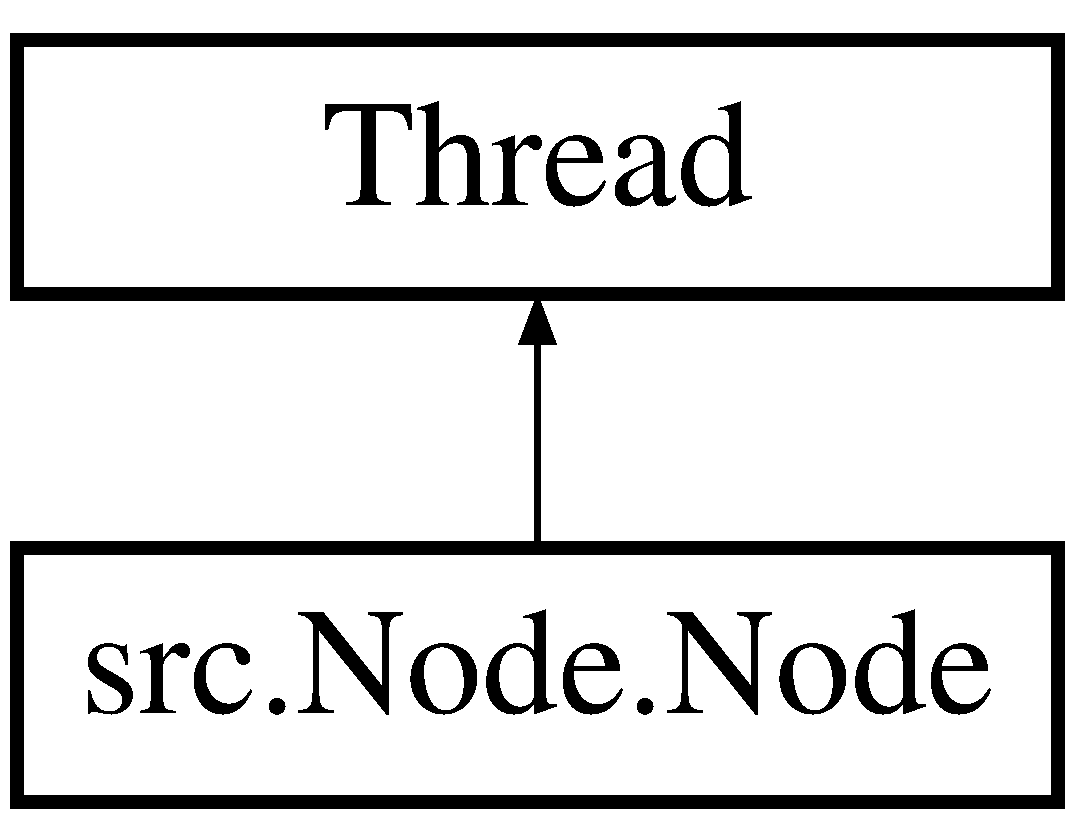
\includegraphics[height=2.000000cm]{classsrc_1_1_node_1_1_node}
\end{center}
\end{figure}
\subsection*{Public Member Functions}
\begin{DoxyCompactItemize}
\item 
\mbox{\Hypertarget{classsrc_1_1_node_1_1_node_aaa2312f4ae71066c441c75e623a5272b}\label{classsrc_1_1_node_1_1_node_aaa2312f4ae71066c441c75e623a5272b}} 
def {\bfseries \+\_\+\+\_\+init\+\_\+\+\_\+} (self, config\+Path)
\item 
def \mbox{\hyperlink{classsrc_1_1_node_1_1_node_a57c5c681b709272de35533e1c02ef394}{stop}} (self)
\item 
def \mbox{\hyperlink{classsrc_1_1_node_1_1_node_a802978364e02620c7c74515b21f14654}{stopped}} (self)
\item 
def \mbox{\hyperlink{classsrc_1_1_node_1_1_node_a362a8826afeeb04d85aed9e0c9f82e22}{run}} (self)
\item 
def \mbox{\hyperlink{classsrc_1_1_node_1_1_node_a8041d0079f6d0526756bc037a6c8a802}{stopzmq}} (self)
\item 
\mbox{\Hypertarget{classsrc_1_1_node_1_1_node_a5258d33ae4917f2b14eb9cca1b20580f}\label{classsrc_1_1_node_1_1_node_a5258d33ae4917f2b14eb9cca1b20580f}} 
def {\bfseries savedata} (self)
\item 
\mbox{\Hypertarget{classsrc_1_1_node_1_1_node_a0474ce7ae845f0686b03dfdef3615d4a}\label{classsrc_1_1_node_1_1_node_a0474ce7ae845f0686b03dfdef3615d4a}} 
def {\bfseries loaddata} (self)
\item 
\mbox{\Hypertarget{classsrc_1_1_node_1_1_node_a5b226b15006ad082b63316cdd6f29f79}\label{classsrc_1_1_node_1_1_node_a5b226b15006ad082b63316cdd6f29f79}} 
def {\bfseries restart} (self)
\item 
def \mbox{\hyperlink{classsrc_1_1_node_1_1_node_a0dd2a9b337a3c3d8ae91178043f60230}{shutdown}} (self)
\item 
def \mbox{\hyperlink{classsrc_1_1_node_1_1_node_a0c82a88ce23ea5b4a117fb91f72a14dd}{loop}} (self)
\item 
def \mbox{\hyperlink{classsrc_1_1_node_1_1_node_a28f03366fdb99400001080178be63525}{initzmq}} (self)
\item 
def \mbox{\hyperlink{classsrc_1_1_node_1_1_node_a901953eab0e8459816753b0dab20853f}{send}} (self, topic, msg)
\item 
def \mbox{\hyperlink{classsrc_1_1_node_1_1_node_a3ca4283da7b7b918412cfffd3833e26d}{recv}} (self, topic, callback)
\item 
def \mbox{\hyperlink{classsrc_1_1_node_1_1_node_ac92e0c1099d7fc66a6a2506ea03407d1}{request}} (self, topic, req, callback)
\item 
def \mbox{\hyperlink{classsrc_1_1_node_1_1_node_a6fee164df1e6f3664f41199258c96810}{reply}} (self, topic, callback)
\end{DoxyCompactItemize}
\subsection*{Public Attributes}
\begin{DoxyCompactItemize}
\item 
\mbox{\Hypertarget{classsrc_1_1_node_1_1_node_aa709af7372ee1d8b16b8a4b583797fbc}\label{classsrc_1_1_node_1_1_node_aa709af7372ee1d8b16b8a4b583797fbc}} 
{\bfseries config\+Path}
\item 
\mbox{\Hypertarget{classsrc_1_1_node_1_1_node_ab86465c66479a6e188cd896e73e7c4d9}\label{classsrc_1_1_node_1_1_node_ab86465c66479a6e188cd896e73e7c4d9}} 
{\bfseries config\+Data}
\item 
\mbox{\Hypertarget{classsrc_1_1_node_1_1_node_a3b5886ac2b9f9aa3312cb5ed51d24e94}\label{classsrc_1_1_node_1_1_node_a3b5886ac2b9f9aa3312cb5ed51d24e94}} 
{\bfseries id}
\item 
\mbox{\Hypertarget{classsrc_1_1_node_1_1_node_aa95cc469e47c4a0a91be78f455ca9076}\label{classsrc_1_1_node_1_1_node_aa95cc469e47c4a0a91be78f455ca9076}} 
{\bfseries context}
\item 
\mbox{\Hypertarget{classsrc_1_1_node_1_1_node_a42eedcf5673b8f2285da2d4ce0f4316d}\label{classsrc_1_1_node_1_1_node_a42eedcf5673b8f2285da2d4ce0f4316d}} 
{\bfseries topics}
\item 
\mbox{\Hypertarget{classsrc_1_1_node_1_1_node_abc9e6fffd4ae8b4c2afa39bfd1c77347}\label{classsrc_1_1_node_1_1_node_abc9e6fffd4ae8b4c2afa39bfd1c77347}} 
{\bfseries status}
\end{DoxyCompactItemize}


\subsection{Detailed Description}
\begin{DoxyVerb}This is the class that will be the base of every node object

Each node will read a config file in JSON format to initialize zmq sockets.
The sockets will be stored in a dict with the key being the topic and the value being the socket
To create a node, make a config file and extend the run() method.
Further functionality is on the way.
\end{DoxyVerb}
 

\subsection{Member Function Documentation}
\mbox{\Hypertarget{classsrc_1_1_node_1_1_node_a28f03366fdb99400001080178be63525}\label{classsrc_1_1_node_1_1_node_a28f03366fdb99400001080178be63525}} 
\index{src\+::\+Node\+::\+Node@{src\+::\+Node\+::\+Node}!initzmq@{initzmq}}
\index{initzmq@{initzmq}!src\+::\+Node\+::\+Node@{src\+::\+Node\+::\+Node}}
\subsubsection{\texorpdfstring{initzmq()}{initzmq()}}
{\footnotesize\ttfamily def src.\+Node.\+Node.\+initzmq (\begin{DoxyParamCaption}\item[{}]{self }\end{DoxyParamCaption})}

\begin{DoxyVerb}This method initializes zmq sockets and places them in the topics dict

It will throw exceptions if the JSON it was fed is not correct
\end{DoxyVerb}
 \mbox{\Hypertarget{classsrc_1_1_node_1_1_node_a0c82a88ce23ea5b4a117fb91f72a14dd}\label{classsrc_1_1_node_1_1_node_a0c82a88ce23ea5b4a117fb91f72a14dd}} 
\index{src\+::\+Node\+::\+Node@{src\+::\+Node\+::\+Node}!loop@{loop}}
\index{loop@{loop}!src\+::\+Node\+::\+Node@{src\+::\+Node\+::\+Node}}
\subsubsection{\texorpdfstring{loop()}{loop()}}
{\footnotesize\ttfamily def src.\+Node.\+Node.\+loop (\begin{DoxyParamCaption}\item[{}]{self }\end{DoxyParamCaption})}

\begin{DoxyVerb}The main node code that gets executed every loop

This is the method that should be overridden for the node to do stuff
So help me God if anyone overrides this and puts a while true in there
\end{DoxyVerb}
 \mbox{\Hypertarget{classsrc_1_1_node_1_1_node_a3ca4283da7b7b918412cfffd3833e26d}\label{classsrc_1_1_node_1_1_node_a3ca4283da7b7b918412cfffd3833e26d}} 
\index{src\+::\+Node\+::\+Node@{src\+::\+Node\+::\+Node}!recv@{recv}}
\index{recv@{recv}!src\+::\+Node\+::\+Node@{src\+::\+Node\+::\+Node}}
\subsubsection{\texorpdfstring{recv()}{recv()}}
{\footnotesize\ttfamily def src.\+Node.\+Node.\+recv (\begin{DoxyParamCaption}\item[{}]{self,  }\item[{}]{topic,  }\item[{}]{callback }\end{DoxyParamCaption})}

\begin{DoxyVerb}This method is used to receive messages for the sub pattern

The first argument is the topic to look for messages on.
The second argument is a function to be executed with the message received being passed to it as an argument
NOT VERIFIED: This method is blocking, and will interrupt execution until a message is received
\end{DoxyVerb}
 \mbox{\Hypertarget{classsrc_1_1_node_1_1_node_a6fee164df1e6f3664f41199258c96810}\label{classsrc_1_1_node_1_1_node_a6fee164df1e6f3664f41199258c96810}} 
\index{src\+::\+Node\+::\+Node@{src\+::\+Node\+::\+Node}!reply@{reply}}
\index{reply@{reply}!src\+::\+Node\+::\+Node@{src\+::\+Node\+::\+Node}}
\subsubsection{\texorpdfstring{reply()}{reply()}}
{\footnotesize\ttfamily def src.\+Node.\+Node.\+reply (\begin{DoxyParamCaption}\item[{}]{self,  }\item[{}]{topic,  }\item[{}]{callback }\end{DoxyParamCaption})}

\begin{DoxyVerb}This method is used to send a reply to a node

The first argument is the topic(in this case, the node) to reply to
The second argument is a callback that will handle the request sent to this node. It must return a string.
The reply generated by the callback is sent as a reply to the node that sent a request
\end{DoxyVerb}
 \mbox{\Hypertarget{classsrc_1_1_node_1_1_node_ac92e0c1099d7fc66a6a2506ea03407d1}\label{classsrc_1_1_node_1_1_node_ac92e0c1099d7fc66a6a2506ea03407d1}} 
\index{src\+::\+Node\+::\+Node@{src\+::\+Node\+::\+Node}!request@{request}}
\index{request@{request}!src\+::\+Node\+::\+Node@{src\+::\+Node\+::\+Node}}
\subsubsection{\texorpdfstring{request()}{request()}}
{\footnotesize\ttfamily def src.\+Node.\+Node.\+request (\begin{DoxyParamCaption}\item[{}]{self,  }\item[{}]{topic,  }\item[{}]{req,  }\item[{}]{callback }\end{DoxyParamCaption})}

\begin{DoxyVerb}This method is used to send a request to a node

The first argument is the topic(in this case, the node) to send a request to.
The second argument is the request to send
The third argument is a callback function to process the reply from the server. The reply will be a string
\end{DoxyVerb}
 \mbox{\Hypertarget{classsrc_1_1_node_1_1_node_a362a8826afeeb04d85aed9e0c9f82e22}\label{classsrc_1_1_node_1_1_node_a362a8826afeeb04d85aed9e0c9f82e22}} 
\index{src\+::\+Node\+::\+Node@{src\+::\+Node\+::\+Node}!run@{run}}
\index{run@{run}!src\+::\+Node\+::\+Node@{src\+::\+Node\+::\+Node}}
\subsubsection{\texorpdfstring{run()}{run()}}
{\footnotesize\ttfamily def src.\+Node.\+Node.\+run (\begin{DoxyParamCaption}\item[{}]{self }\end{DoxyParamCaption})}

\begin{DoxyVerb}This will be the node's main loop

Everyone should override the loop and shutdown methods.
\end{DoxyVerb}
 \mbox{\Hypertarget{classsrc_1_1_node_1_1_node_a901953eab0e8459816753b0dab20853f}\label{classsrc_1_1_node_1_1_node_a901953eab0e8459816753b0dab20853f}} 
\index{src\+::\+Node\+::\+Node@{src\+::\+Node\+::\+Node}!send@{send}}
\index{send@{send}!src\+::\+Node\+::\+Node@{src\+::\+Node\+::\+Node}}
\subsubsection{\texorpdfstring{send()}{send()}}
{\footnotesize\ttfamily def src.\+Node.\+Node.\+send (\begin{DoxyParamCaption}\item[{}]{self,  }\item[{}]{topic,  }\item[{}]{msg }\end{DoxyParamCaption})}

\begin{DoxyVerb}This method can be used to send messages for the pub pattern

The first argument is the topic to send the message on and the second is the message body
\end{DoxyVerb}
 \mbox{\Hypertarget{classsrc_1_1_node_1_1_node_a0dd2a9b337a3c3d8ae91178043f60230}\label{classsrc_1_1_node_1_1_node_a0dd2a9b337a3c3d8ae91178043f60230}} 
\index{src\+::\+Node\+::\+Node@{src\+::\+Node\+::\+Node}!shutdown@{shutdown}}
\index{shutdown@{shutdown}!src\+::\+Node\+::\+Node@{src\+::\+Node\+::\+Node}}
\subsubsection{\texorpdfstring{shutdown()}{shutdown()}}
{\footnotesize\ttfamily def src.\+Node.\+Node.\+shutdown (\begin{DoxyParamCaption}\item[{}]{self }\end{DoxyParamCaption})}

\begin{DoxyVerb}Gets called when the node is told to stop

Everyone should override this for good practice
\end{DoxyVerb}
 \mbox{\Hypertarget{classsrc_1_1_node_1_1_node_a57c5c681b709272de35533e1c02ef394}\label{classsrc_1_1_node_1_1_node_a57c5c681b709272de35533e1c02ef394}} 
\index{src\+::\+Node\+::\+Node@{src\+::\+Node\+::\+Node}!stop@{stop}}
\index{stop@{stop}!src\+::\+Node\+::\+Node@{src\+::\+Node\+::\+Node}}
\subsubsection{\texorpdfstring{stop()}{stop()}}
{\footnotesize\ttfamily def src.\+Node.\+Node.\+stop (\begin{DoxyParamCaption}\item[{}]{self }\end{DoxyParamCaption})}

\begin{DoxyVerb}This method sets the stop flag

The node should safely shut down after this flag is set
\end{DoxyVerb}
 \mbox{\Hypertarget{classsrc_1_1_node_1_1_node_a802978364e02620c7c74515b21f14654}\label{classsrc_1_1_node_1_1_node_a802978364e02620c7c74515b21f14654}} 
\index{src\+::\+Node\+::\+Node@{src\+::\+Node\+::\+Node}!stopped@{stopped}}
\index{stopped@{stopped}!src\+::\+Node\+::\+Node@{src\+::\+Node\+::\+Node}}
\subsubsection{\texorpdfstring{stopped()}{stopped()}}
{\footnotesize\ttfamily def src.\+Node.\+Node.\+stopped (\begin{DoxyParamCaption}\item[{}]{self }\end{DoxyParamCaption})}

\begin{DoxyVerb}Returns the value of the stopped flag\end{DoxyVerb}
 \mbox{\Hypertarget{classsrc_1_1_node_1_1_node_a8041d0079f6d0526756bc037a6c8a802}\label{classsrc_1_1_node_1_1_node_a8041d0079f6d0526756bc037a6c8a802}} 
\index{src\+::\+Node\+::\+Node@{src\+::\+Node\+::\+Node}!stopzmq@{stopzmq}}
\index{stopzmq@{stopzmq}!src\+::\+Node\+::\+Node@{src\+::\+Node\+::\+Node}}
\subsubsection{\texorpdfstring{stopzmq()}{stopzmq()}}
{\footnotesize\ttfamily def src.\+Node.\+Node.\+stopzmq (\begin{DoxyParamCaption}\item[{}]{self }\end{DoxyParamCaption})}

\begin{DoxyVerb}Shuts down all zmq stuff\end{DoxyVerb}
 

The documentation for this class was generated from the following file\+:\begin{DoxyCompactItemize}
\item 
Node.\+py\end{DoxyCompactItemize}

\hypertarget{classsrc_1_1status_1_1_status}{}\section{src.\+status.\+Status Class Reference}
\label{classsrc_1_1status_1_1_status}\index{src.\+status.\+Status@{src.\+status.\+Status}}
Inheritance diagram for src.\+status.\+Status\+:\begin{figure}[H]
\begin{center}
\leavevmode
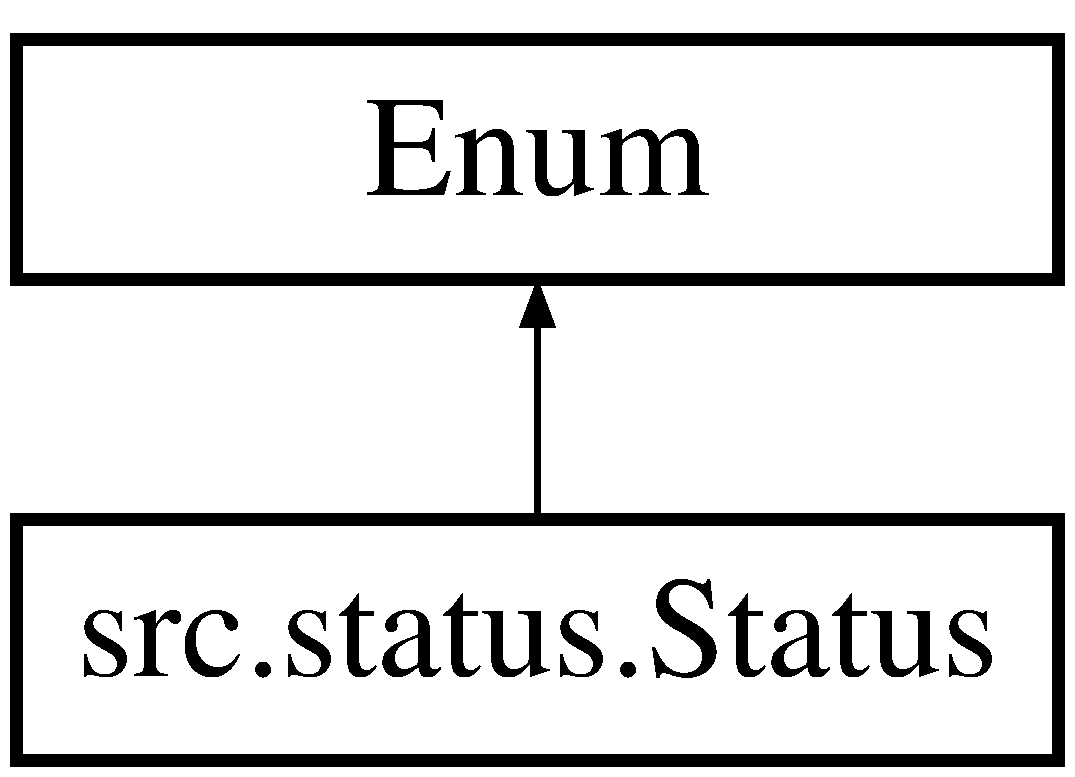
\includegraphics[height=2.000000cm]{classsrc_1_1status_1_1_status}
\end{center}
\end{figure}
\subsection*{Static Public Attributes}
\begin{DoxyCompactItemize}
\item 
\mbox{\Hypertarget{classsrc_1_1status_1_1_status_a0677342a89262926ba4b62e5ee45d18e}\label{classsrc_1_1status_1_1_status_a0677342a89262926ba4b62e5ee45d18e}} 
int {\bfseries R\+U\+N\+N\+I\+NG} = 0
\item 
\mbox{\Hypertarget{classsrc_1_1status_1_1_status_ab83b5d2ef99371968c6ddafcee0d9d60}\label{classsrc_1_1status_1_1_status_ab83b5d2ef99371968c6ddafcee0d9d60}} 
int {\bfseries F\+I\+N\+I\+S\+H\+ED} = 1
\item 
\mbox{\Hypertarget{classsrc_1_1status_1_1_status_ad2701177cd592015f2d425889dbec315}\label{classsrc_1_1status_1_1_status_ad2701177cd592015f2d425889dbec315}} 
int {\bfseries C\+R\+A\+S\+H\+ED} = 2
\item 
\mbox{\Hypertarget{classsrc_1_1status_1_1_status_af9f5483bfd7a5534cb7b7f786324bbda}\label{classsrc_1_1status_1_1_status_af9f5483bfd7a5534cb7b7f786324bbda}} 
int {\bfseries S\+T\+O\+P\+P\+ED} = 3
\end{DoxyCompactItemize}


The documentation for this class was generated from the following file\+:\begin{DoxyCompactItemize}
\item 
status.\+py\end{DoxyCompactItemize}

%--- End generated contents ---

% Index
\backmatter
\newpage
\phantomsection
\clearemptydoublepage
\addcontentsline{toc}{chapter}{Index}
\printindex

\end{document}
